\documentclass[tikz, landscape]{standalone}
\usepackage[charter]{mathdesign}
\usetikzlibrary{arrows, arrows.meta, automata, positioning}
\tikzset{larrow/.style = {-{Latex[length=.5em]}}}

\begin{document}
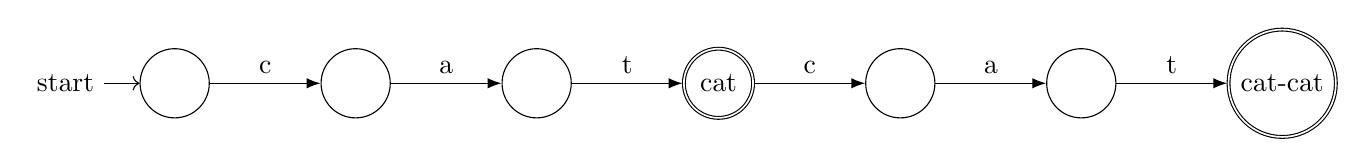
\begin{tikzpicture}
    \node[state,initial]   (0) at (0,0) {};
    \node[state]           (1) [right=4em of 0] {};
    \node[state]           (2) [right=4em of 1] {};
    \node[state,accepting] (3) [right=4em of 2] {cat};
    \node[state]           (4) [right=4em of 3] {};
    \node[state]           (5) [right=4em of 4] {};
    \node[state,accepting] (6) [right=4em of 5] {cat-cat};

    \foreach \State/\Label [remember=\State as \lastState (initially 0)] in {%
        1/c,
        2/a,
        3/t,
        4/c,
        5/a,
        6/t%
    }
    \draw[larrow] (\lastState) to node [above] {\Label} (\State);
\end{tikzpicture}
\end{document}
